\documentclass[11pt,letterpaper]{article}
% Submission layout follows the official STOC 2027 CFP.
% The manuscript was developed from the supplied local ACM template;
% the ACM bibliography style is retained, and the submission layout is adapted.
\usepackage[letterpaper,margin=1in]{geometry}
\usepackage[T1]{fontenc}
\usepackage{libertine}
\usepackage{amsmath,amsthm,mathtools,booktabs,array,enumitem,graphicx}
\usepackage{newtxmath}
\usepackage{cite}
\usepackage[unicode,colorlinks=true,linkcolor=blue!55!black,citecolor=blue!55!black,urlcolor=blue!55!black]{hyperref}
\usepackage{microtype}
\newcolumntype{P}[1]{>{\raggedright\arraybackslash}p{#1}}
\usepackage{tikz}
\usetikzlibrary{arrows.meta,positioning,fit,backgrounds,calc}
\usepackage{caption}
\usepackage{attachfile2}
\captionsetup{font=normalsize,labelfont=bf}
\setlength{\parskip}{0pt}
\setlength{\parindent}{1em}
\newcommand{\Description}[1]{}
\newtheorem{theorem}{Theorem}
\newtheorem{lemma}[theorem]{Lemma}
\newtheorem{corollary}[theorem]{Corollary}
\newtheorem{proposition}[theorem]{Proposition}
\theoremstyle{definition}
\newtheorem{definition}[theorem]{Definition}
\newcommand{\Bool}{\{0,1\}}
\newcommand{\Omv}{\mathsf{OMv}}
\newcommand{\SC}{\mathsf{SC}}
\newcommand{\VP}{\mathsf{VP}}
\newcommand{\tw}{\operatorname{tw}}
\newcommand{\cost}{\mathcal C_\eta}
\newcommand{\TreeFlow}{\textsc{TreeFlow}}
\newcommand{\poly}{\operatorname{poly}}
\newcommand{\Rel}{\mathsf R}
\newcommand{\bits}{\mathsf{bits}}
\newcommand{\supp}{\operatorname{supp}}
\newcommand{\cl}{\operatorname{cl}}
\newcommand{\zero}{\mathbf 0}
\newcommand{\Id}{\mathbf I}
\definecolor{tfblue}{RGB}{27,78,119}
\definecolor{tfgreen}{RGB}{20,106,92}
\definecolor{tforange}{RGB}{151,80,20}
\tikzset{box/.style={draw=tfblue,rounded corners=2pt,fill=blue!3,align=center,inner sep=6pt,font=\normalsize},
 arr/.style={-{Stealth[length=2mm]},thick,draw=tfblue},
 point/.style={circle,draw=tfblue,fill=blue!4,minimum size=5mm,inner sep=1pt,font=\normalsize}}
\hypersetup{
 pdftitle={Fully Dynamic Interprocedural Dataflow Analysis: OMv Barriers and Summary-Local TreeFlow Updates},
 pdfauthor={Zijian Zeng; Jiayin Cao; Weinan Dai; Rui Wang; Fei Ding}}
\begin{document}
\begin{titlepage}
\thispagestyle{empty}
\begin{center}
{\LARGE\bfseries Fully Dynamic Interprocedural Dataflow Analysis:\par
\vspace{5pt}
OMv Barriers and Summary-Local TreeFlow Updates\par}
\vspace{18pt}
{\large Zijian Zeng}\\
UCSI University\\
\href{mailto:1002266693@ucsiuniversity.edu.my}{1002266693@ucsiuniversity.edu.my}\\[9pt]
{\large Jiayin Cao}\\
Ningbo University\\
\href{mailto:2795820153@qq.com}{2795820153@qq.com}\\[9pt]
{\large Weinan Dai}\\
Zhejiang University\\
\href{mailto:21725058@zju.edu.cn}{21725058@zju.edu.cn}\\[9pt]
{\large Rui Wang}\\
Nanchang Institute of Technology\\
\href{mailto:2002007@nut.edu.cn}{2002007@nut.edu.cn}\\[9pt]
{\large Fei Ding}\\
Alibaba Group\\
\href{mailto:dingfei@email.ncu.edu.cn}{dingfei@email.ncu.edu.cn}
\end{center}
\vspace{10pt}
\noindent\textbf{Abstract.}\quad
Can bounded treewidth make interprocedural dataflow analysis respond to
every program edit in subpolynomial time? We show why a restriction on
individual control-flow graphs is insufficient. Assuming the online
Boolean matrix--vector multiplication conjecture, no fully dynamic IFDS
algorithm with polynomial preprocessing has both $n^{1-\varepsilon}$
update and query time, even when every procedure is a path, there is one
nonzero fact, and the call graph is acyclic of depth one. The obstruction
is shared callee summaries at multi-target call sites, rather than
recursion. Independently, a three-vertex, one-procedure path yields the
analogous $D^{1-\varepsilon}$ barrier for elementary flow-relation edits.
Both barriers are tight for their matrix--selector subfamilies.

We give a positive theorem with an explicit missing parameter:
the number $\lambda$ of summary-circuit gates affected by an edit.
On supplied binary decompositions of width $t$ and height $H$, and an
acyclic candidate call graph, TreeFlow preprocesses in
$O(S((t+5)(D+1))^{\omega+\eta})$ time and updates in
$O(\lambda((t+5)(D+1))^{\omega+\eta})$ time, for every $\eta>0$;
$S$ is the circuit size. Same-context fact queries cost
$O(H((t+5)(D+1))^{\omega+\eta})$.

An ancestor-incidence bound gives polylogarithmic updates with shared
callees, including a chain of call diamonds with exponentially many call
paths. Complete proofs separate local computation, matched calls, and
global propagation. Executable source and per-comparison traces are embedded
in the PDF; validation concerns finite correctness, not repository latency.
\end{titlepage}
\setcounter{page}{1}
\pagestyle{plain}

\section{Introduction}
An edit to a branch, assignment, or call target can invalidate an IDE's
interprocedural taint, possible-nullness, or uninitialized-variable analysis.
The IFDS framework solves finite distributive may-analyses by following fact
paths with matching calls and returns, with classical static cost $O(ED^3)$
\cite{RHS95}. Structured intraprocedural control flow has small treewidth
\cite{Thorup98}, making local dynamic programming attractive. The central
question is whether this local structure also controls global update cost.

Our main result isolates an obstruction: \emph{shared callee summaries encode
arbitrary matrix incidence even when every procedure is a path}. The call
graph can be acyclic of depth one, with one ordinary fact. A leaf-edge edit
then implements one online-vector selector, and caller entry-to-exit queries
recover the matrix--vector product. Thus small local treewidth and shallow
calls together still permit OMv hardness. Figure~\ref{fig:calls} shows the
construction. The relevant missing structure is the size of the caller
incidence region reached by an edit.

TreeFlow separates these two sources of work. It compiles fixed local
decompositions and an acyclic candidate call graph into a relation circuit.
Bag closures enforce local reachability; site-specific products enforce
matching calls and returns. The circuit supports deletion as well as
insertion by recomputing affected gates from their current inputs. We bound
its propagation volume by a \emph{program-level ancestor-incidence parameter},
including programs with exponentially many call paths but only logarithmically
many affected call occurrences.

\subsection{Results and normalization}
On a word RAM, let $n$ count program points, $D$ ordinary facts, and
$d=D+1$ include the zero fact. The full size $L$ counts explicit target
and relation entries; $\bits(e)$ charges the edit payload in that representation. All preprocessing lower bounds allow $\poly(L)$
time. Dense reductions have $n=\Theta(k)$ but $L=O(k^2)$; with padding,
$L=\Theta(k^2)$. Their near-linear $n$ barrier therefore becomes a
square-root barrier in $L$. This normalization is part of the statements.
Write $\cost(q)=O(q^{\omega+\eta})$ for Boolean multiplication or closure,
for any fixed $\eta>0$.

\begin{theorem}[Program-point barrier]\label{thm:n}
Assume OMv. For every constant $\varepsilon>0$, polynomial preprocessing
cannot support both amortized update and Boolean membership-query time
$O(n^{1-\varepsilon})$ for fully dynamic IFDS, even with one procedure,
$D=1$, a fixed source fact, and identity-edge insertions/deletions.
\end{theorem}

\begin{theorem}[Path-procedure barrier]\label{thm:calls}
Assume OMv. The same exclusion holds for same-context point-to-point queries
when every local procedure skeleton is a path, $D=1$, call/return transfers
are fixed identities, and the candidate call graph is acyclic of depth one.
Each procedure has at most one call site, possibly with multiple targets.
Only a leaf procedure's normal edge changes. There are $\Theta(n)$
procedures and $O(n^2)$ target occurrences.
\end{theorem}

Consequently, per-procedure treewidth alone cannot imply updates
$f(t)n^{o(1)}D^\omega$ with queries $O(D\log n)$ in this model.

\begin{theorem}[Fact-domain barrier]\label{thm:d}
Assume OMv. Polynomial preprocessing cannot support both update and Boolean
membership-query time $O(D^{1-\varepsilon})$ for any constant
$\varepsilon>0$, even on a fixed three-point path in one procedure. An
update changes one pair in one transfer relation; the source fact and a
second, matrix-encoding relation remain fixed.
\end{theorem}

For the positive results, supply rooted binary local decompositions of
width $t$ and height $H\ge1$, counting bags along a root-to-leaf path.
Their candidate skeletons cover all allowed local edges and call interfaces.
The candidate call graph is acyclic. Let $S$ be the compiled circuit size,
$K=(t+5)d$, and $\lambda(e)$ count internal gates reachable from the
input leaves changed by edit $e$.

\begin{theorem}[Certified TreeFlow]\label{thm:upper}
TreeFlow uses $O(SK^2)$ space and $O(S\cost(K))$ preprocessing. A legal
edge/target activation, deactivation, or transfer edit costs
$O(\bits(e)+1+\lambda(e)\cost(K))$ worst-case time, where $\bits(e)$
charges the supplied payload. Same-context fact membership within a
procedure costs $O(H\cost(K))$; entry-to-exit membership costs $O(1)$.
\end{theorem}

Orient each candidate target occurrence from its callee to its caller,
retaining parallel occurrences. Let $A(p)$ contain $p$ and all procedures
reachable from $p$ in this multigraph, and let $a(p)$ count occurrences
whose callee lies in $A(p)$. Their callers automatically lie in $A(p)$.
For an edit to a target or call/return transfer, $p$ denotes its containing
caller; for a local-edge edit, it denotes the edited procedure.

\begin{corollary}[Ancestor-incidence bound]\label{cor:sharing}
Under Theorem~\ref{thm:upper}, an elementary edit in $p$ satisfies
\[
 \lambda(e)=O\bigl((1+a(p))(H+\log(S+2))\bigr).
\]
For fixed $t,D$, logarithmic $H$, polynomial $S$, and
$a(p)=\log^{O(1)}n$, updates are polylogarithmic even with shared callees.
\end{corollary}

\begin{corollary}[Unique occurrence]\label{cor:forest}
If each procedure is the callee of at most one candidate target occurrence
and call depth is $h$, then $a(p)\le h$. For fixed $t,D$ and
$h,H=O(\log n)$, updates take $O(\log^2 n)$ and same-context queries
$O(\log n)$ time.
\end{corollary}

A chain of $r$ call diamonds illustrates the stronger corollary: $A_i$
can call $B_i$ or $C_i$, and both call $A_{i+1}$. There are $2^r$
call paths to $A_r$ but only $4r$ candidate occurrences in its ancestor
region. Each local skeleton is a path. Recursive interval bags containing two
endpoints and a midpoint give width two and logarithmic height. Padding
paths within procedures sets the total size $n$; for $r=O(\log n)$,
Corollary~\ref{cor:sharing} gives polylogarithmic updates with shared callees.

\subsection{Technical overview and relation to prior work}
Theorem~\ref{thm:calls} places dense matrix incidence \emph{between}
procedures while preserving every local path skeleton. The other two
reductions place it in ordinary CFG edges or in a single fact relation.
All use $O(k)$ selector edits and $k$ row queries per online vector.

TreeFlow maintains reachability among bag-boundary/fact states, of order
$O((t+1)d)$. Child summaries are combined by union and reflexive transitive
closure, accounting for repeated alternations between regions. A completed
call contributes $C_{s,p}S_pR_{s,p}$ to its own return site, and a balanced
union tree aggregates alternative callees. Call-graph acyclicity makes the
whole dependency circuit acyclic. Figure~\ref{fig:framework} separates local
recomputation, propagation to other procedures, and query access.

The local machinery has important antecedents. Theorem~3.8 of
\cite{CGGIP19} supports local edge-weight updates in $O(\log n)$ semiring
operations; its global RSM computation repeatedly updates box summaries,
and Corollary~4.5 gives the static IFDS query oracle in
Table~\ref{tab:comparison}. TreeFlow reuses separator dynamic programming
and affected-DAG recomputation. Its program-specific guarantees are the
explicit compilation for target/transfer edits, the incidence obstruction
of Theorem~\ref{thm:calls}, and the bound of Corollary~\ref{cor:sharing},
which counts shared occurrences once irrespective of the number of call
paths. These results distinguish global maintenance from an update to one
already-summarized local graph. Static optimized same-context queries
\cite{CGIP20} remain faster than our simple pinning oracle.

\begin{table}[t]
\centering
\caption{Quantitative comparison. $b$ counts RSM boxes; $\tau$ is the
per-bag automaton cost. Costs apply to the tasks indicated.}
\label{tab:comparison}
\begin{tabular}{P{3.4cm}P{6.0cm}P{5.5cm}}
\toprule
Setting & Cost & Scope\\
\midrule
IFDS \cite{RHS95} & $O(ED^3)$ & Static complete solve\\
RSMs \cite{CGGIP19} & $O((n+b\log n)D^3)$ build; $O(D^2\log n)$ query & Static same-context oracle\\
Incremental systems\newline\cite{AB14,MNPH15,MMII13} & Work follows invalidated derivations or dataflow differences & No local-treewidth bound on global IFDS edits stated\\
Dynamic treewidth\newline\cite{Korhonen25} & $2^{O(t)}\tau(9t+8)\log n$ amortized update & Decomposition and supplied automaton\\
TreeFlow & $O(SK^{\omega+\eta})$ build; $O(\bits(e)+1+\lambda K^{\omega+\eta})$ update & Fixed certificates, acyclic calls\\
OMv barriers & Exclude $U,Q=O(n^{1-\varepsilon})$ or $O(D^{1-\varepsilon})$ & Path procedures or one three-point path\\
\bottomrule
\end{tabular}
\end{table}

\begin{figure}[t]
\centering
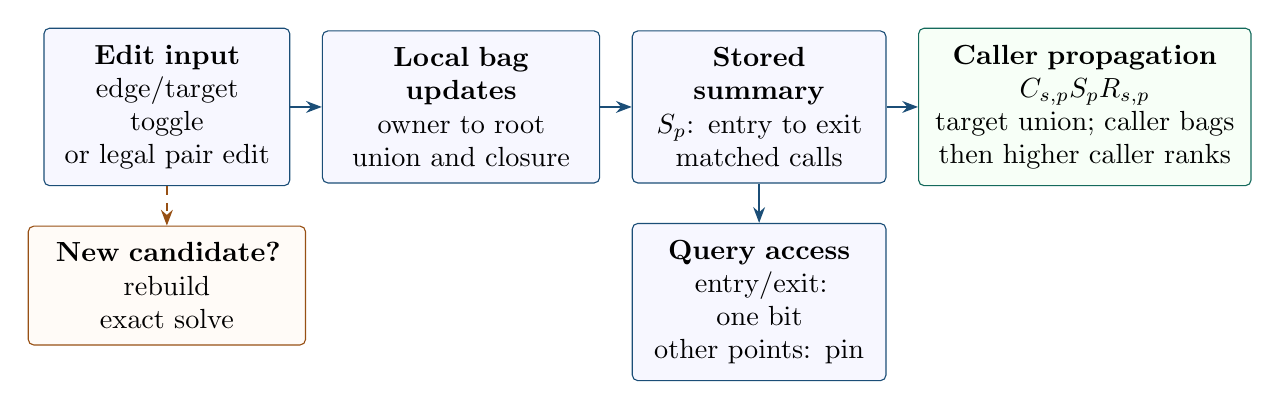
\begin{tikzpicture}[node distance=5mm and 4mm]
\node[box,text width=2.7cm] (e) {\textbf{Edit input}\\edge/target toggle\\or legal pair edit};
\node[box,text width=3.1cm,right=of e] (b) {\textbf{Local bag updates}\\owner to root\\union and closure};
\node[box,text width=2.8cm,right=of b] (s) {\textbf{Stored summary}\\$S_p$: entry to exit\\matched calls};
\node[box,text width=3.8cm,right=of s,draw=tfgreen,fill=green!3] (c) {\textbf{Caller propagation}\\$C_{s,p}S_pR_{s,p}$\\target union; caller bags\\then higher caller ranks};
\node[box,text width=3.1cm,below=of e,draw=tforange,fill=orange!3] (f) {\textbf{New candidate?}\\rebuild\\exact solve};
\node[box,text width=2.8cm,below=of s] (q) {\textbf{Query access}\\entry/exit: one bit\\other points: pin};
\draw[arr] (e)--(b);\draw[arr] (b)--(s);\draw[arr] (s)--(c);
\draw[arr] (s)--(q);\draw[arr,dashed,draw=tforange] (e)--(f);
\end{tikzpicture}
\caption{TreeFlow's acyclic update stages. Caller propagation moves strictly
up the call DAG; it does not feed back into the edited procedure. Queries
read maintained summaries on a separate branch. Bag matrices have order
$O((t+1)d)$, $d=D+1$; an edit reaches $\lambda$ gates, costing
$O(\bits(e)+1+\lambda\cost((t+5)d))$.}
\label{fig:framework}
\end{figure}


\section{Model}\label{sec:model}
Each procedure has entry $e_p$, exit $x_p$, and disjoint point set $V_p$.
A call site $s$ has call point $c_s$, return point $r_s$, and candidate
callees. Selecting $p$ pushes $(s,p)$; its return must pop that same
pair and go to $r_s$. The undirected \emph{local skeleton} contains
normal edges and each structural interface edge $\{c_s,r_s\}$. The
interface edge itself need not have executable bypass flow.

A union-distributive map satisfies
$f(X)=f(\varnothing)\cup\bigcup_{a\in X}f(\{a\})$ and is represented
on $\widehat{\mathcal F}=\mathcal F\cup\{0\}$ by a Boolean relation.
\emph{Legal active transfers} contain $(0,0)$, contain no $(a,0)$ with
$a\ne0$, and may contain generation pairs $(0,b)$ and propagation
pairs $(a,b)$. These conditions represent exactly a union-distributive
map, allowing redundant propagation pairs. A relation edit preserves these
conditions; pair edits cannot remove $(0,0)$ or create $(a,0)$.
Deactivation removes the entire edge/target contribution, including its
zero transition. Our hardness gadgets generate no ordinary fact from $0$.

$\SC((u,a),(v,b))$ denotes balanced, same-context reachability without
popping the initial stack. Its endpoints are in one procedure.
$\VP$ denotes reachability from an empty stack with unmatched calls
allowed at the end. A membership query returns one Boolean; enumeration
may require $\Omega(nd)$ output.

Points, facts, candidate edges, targets, and certificates are fixed during
a fast-path run. Edits activate/deactivate one edge or paired target,
change one legal relation pair, or replace a relation with its payload.
One source commit may induce many edits and front-end work; costs add.
New candidates or facts require rebuilding. All upper bounds concern IFDS
relations; IDE value lattices require additional representation and
convergence bounds.

\section{OMv lower bounds}\label{sec:lower}
OMv receives a Boolean $k\times k$ matrix and then $k$ online vectors;
each product must be output before the next vector arrives. We invoke
its polynomial-preprocessing consequence \cite[Theorem~2.2]{HKNS15}:
polynomial matrix preprocessing still excludes a truly subcubic online
phase, assuming the usual OMv conjecture.

\begin{lemma}[Selector accounting]\label{lem:selector}
If a size parameter is $z=\Theta(k)$, and each vector is processed by
$O(k)$ updates and $k$ Boolean queries recovering $Mv$, simultaneous
$U,Q=O(z^{1-\varepsilon})$ contradict OMv.
\end{lemma}
\begin{proof}
The $k$ rounds cost $O(k^2(U+Q)+k^2)$, truly subcubic under those bounds.
Amortized costs apply to the full sequence. For randomized structures,
initialize $O(\log k)$ \emph{independently randomized copies}, feed all
copies the same updates, and majority-vote their answers. On a fixed input sequence, constant error
per answer becomes $O(k^{-3})$; a union bound gives bounded error over
$k^2$ answers. The logarithmic overhead preserves a positive polynomial
improvement. This repeats whole data structures, not queries on one
random state. The invoked preprocessing theorem handles any polynomial
initialization cost.
\end{proof}

\begin{proof}[Proof of Theorem~\ref{thm:n}]
Use entry $s$, columns $q_j$, rows $p_i$, and exit $x$ in one procedure.
Fix identity edges $q_j\to p_i$ iff $M_{ij}=1$ and $p_i\to x$ for
all $i$. Activate $s\to q_j$ exactly when $v_j=1$. With ordinary fact
$\bullet$, the layered graph gives
$\SC((s,\bullet),(p_i,\bullet))=(Mv)_i$. There are $2k+2$ points,
$O(k^2)$ edges, at most $k$ toggles per vector, and $k$ fixed-source
queries. Apply Lemma~\ref{lem:selector}.
\end{proof}

\begin{proof}[Proof of Theorem~\ref{thm:calls}]
For row $i$, create $P_i$ with normal identity edges $e_i\to c_i$ and
$r_i\to x_i$. Site $(c_i,r_i)$ has target $Q_j$ iff $M_{ij}=1$,
with identity call/return transfers and no executable bypass. Column
procedure $Q_j$ has just entry $a_j$, exit $b_j$, and selectable identity
edge $a_j\to b_j$, active iff $v_j=1$.

The local skeletons are the paths $e_i-c_i-r_i-x_i$ and $a_j-b_j$.
The candidate call graph contains only $P_i\to Q_j$ arcs. A balanced
path through $P_i$ must choose some $Q_j$, traverse its active edge,
and return to the same site. Hence
\[
 \SC((e_i,\bullet),(x_i,\bullet))=\bigvee_j M_{ij}v_j=(Mv)_i.
\]
The $6k$ points and at most $k^2$ targets are built during preprocessing.
Installing each vector takes at most $k$ leaf-edge edits and $k$
entry-to-exit queries. Lemma~\ref{lem:selector} applies with $z=n$.
\end{proof}

\begin{figure}[t]
\centering
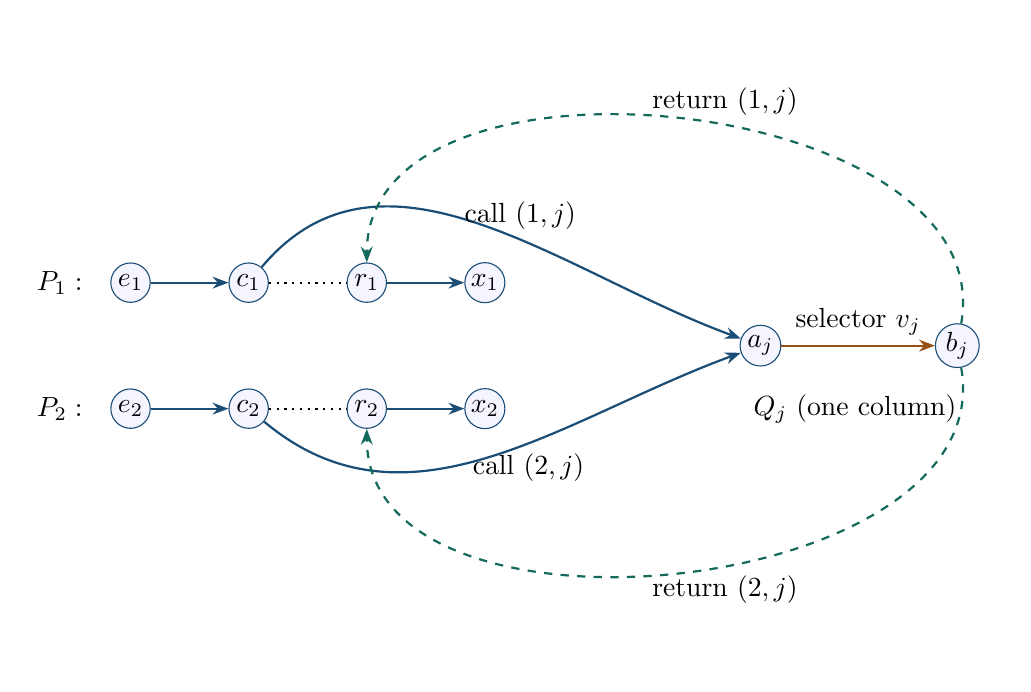
\begin{tikzpicture}[x=1cm,y=1cm]
\foreach \i/\y in {1/0.8,2/-0.8} {
 \node at (-0.9,\y) {$P_{\i}:$};
 \node[point] (e\i) at (0,\y) {$e_{\i}$};
 \node[point] (c\i) at (1.5,\y) {$c_{\i}$};
 \node[point] (r\i) at (3.0,\y) {$r_{\i}$};
 \node[point] (x\i) at (4.5,\y) {$x_{\i}$};
 \draw[arr] (e\i)--(c\i);\draw[arr] (r\i)--(x\i);
 \draw[dotted,thick] (c\i)--(r\i);
}
\node[point] (a) at (8,0) {$a_j$};
\node[point] (b) at (10.5,0) {$b_j$};
\node at (9.2,-0.8) {$Q_j$ (one column)};
\draw[arr,draw=tforange] (a)--node[above] {selector $v_j$}(b);
\draw[arr] (c1) to[out=50,in=160] node[pos=0.58,above] {call $(1,j)$} (a);
\draw[arr] (c2) to[out=-40,in=200] node[pos=0.58,below] {call $(2,j)$} (a);
\draw[arr,dashed,draw=tfgreen] (b) to[out=80,in=90] node[pos=0.45,above] {return $(1,j)$} (r1);
\draw[arr,dashed,draw=tfgreen] (b) to[out=-80,in=-90] node[pos=0.45,below] {return $(2,j)$} (r2);
\end{tikzpicture}
\caption{The path-procedure barrier (Theorem~\ref{thm:calls}). Two of the
$k$ row procedures and one shared column procedure are shown. A target
exists iff $M_{ij}=1$; returns match the labeled call choice. Dotted local
interfaces have no executable bypass. Toggling one orange leaf edge changes
many caller summaries while each local skeleton remains a path.}
\label{fig:calls}
\end{figure}


A root dispatcher that can call every $P_i$ gives a fixed-source $\VP$
version of depth two: its entry reaches $x_i$ iff $(Mv)_i=1$.
For monomorphic calls, give $P_i$ one branch
$e_i\to c_{ij}$, call $Q_j$, $r_{ij}\to x_i$ per matrix entry.
Bags $\{e_i,x_i,c_{ij}\}$ and $\{x_i,c_{ij},r_{ij}\}$ form a
width-two decomposition, joining the first bags. Padding to $\Theta(k^2)$
points gives the corresponding exclusion $U,Q=O(n^{1/2-\varepsilon})$.

\begin{proof}[Proof of Theorem~\ref{thm:d}]
On $s\to a\to z$, use ordinary facts
$\{\sigma,c_1,\ldots,c_k,r_1,\ldots,r_k\}$, so $D=2k+1$.
The first relation $A_v$ contains $(\sigma,c_j)$ iff $v_j=1$; the
fixed second relation $B_M$ contains $(c_j,r_i)$ iff $M_{ij}=1$.
Both also contain $(0,0)$, with no other zero-related pairs. Then
$(A_vB_M)[\sigma,r_i]=\bigvee_j v_jM_{ij}$.
Each vector-coordinate change is one legal pair edit in $A_v$;
query $(s,\sigma)$ to $(z,r_i)$ for each row. Apply
Lemma~\ref{lem:selector} with size parameter $D$. The CFG is always a
three-point path and its matrix relation has $O(D^2)$ entries.
\end{proof}

\begin{figure}[t]
\centering
\begin{minipage}[t]{0.47\linewidth}
\centering
\textbf{(a) Matrix in CFG edges}\par\vspace{5pt}
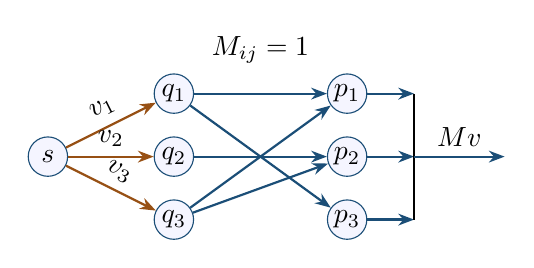
\begin{tikzpicture}[x=1cm,y=1cm]
\node[point] (s) at (0,0) {$s$};
\foreach \j/\y in {1/0.8,2/0,3/-0.8} {
 \node[point] (c\j) at (1.6,\y) {$q_{\j}$};
 \node[point] (r\j) at (3.8,\y) {$p_{\j}$};
 \draw[arr,draw=tforange] (s)--node[above,sloped] {$v_{\j}$}(c\j);
 \draw[arr] (r\j)--(4.65,\y);
}
\draw[thick] (4.65,-0.8)--(4.65,0.8);
\draw[arr] (4.65,0)--node[above] {$Mv$}(5.8,0);
\draw[arr] (c1)--(r1);\draw[arr] (c1)--(r3);
\draw[arr] (c2)--(r2);\draw[arr] (c3)--(r1);\draw[arr] (c3)--(r2);
\node at (2.7,1.35) {$M_{ij}=1$};
\end{tikzpicture}
\end{minipage}\hfill
\begin{minipage}[t]{0.49\linewidth}
\centering
\textbf{(b) Matrix in one transfer}\par\vspace{12pt}
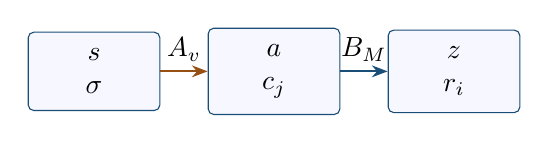
\begin{tikzpicture}[node distance=6mm]
\node[box,text width=1.25cm] (s) {$s$\\$\sigma$};
\node[box,text width=1.25cm,right=of s] (a) {$a$\\$c_j$};
\node[box,text width=1.25cm,right=of a] (z) {$z$\\$r_i$};
\draw[arr,draw=tforange] (s)--node[above] {$A_v$}(a);
\draw[arr] (a)--node[above] {$B_M$}(z);
\end{tikzpicture}\par\vspace{8pt}
$A_v:\sigma\mapsto\{c_j:v_j=1\}$\\
$B_M:c_j\mapsto\{r_i:M_{ij}=1\}$
\end{minipage}
\caption{The other two OMv encodings. Orange selectors change with the
online vector. (a) A query bus collects every row answer; exit edges are
omitted. (b) The CFG has three points and the fixed matrix is one transfer;
each vector bit changes one pair. Both yield $k$ answers equal to $Mv$.}
\label{fig:selectors}
\end{figure}


\begin{proposition}[Tight selector threshold]\label{prop:tight}
For the fixed-matrix selector family in each reduction, $O(k)$ update
and $O(1)$ query time, or $O(1)$ update and $O(k)$ query time, suffice.
\end{proposition}
\begin{proof}
Maintain $c_i=\sum_jM_{ij}v_j$. Toggling $v_j$ changes each count by
$\pm M_{ij}$ in $O(k)$ word operations; answer by $c_i>0$.
Alternatively store $v$ and scan a row per query. Counts fit in
$O(\log k)$ bits. Here $k=\Theta(n)$ in the first two reductions
and $k=\Theta(D)$ in the third.
\end{proof}

\section{TreeFlow and its proof}\label{sec:algorithm}
\subsection{Local summaries and matching}
Root each supplied decomposition and assign each candidate local edge
or interface to one containing bag. Add the procedure entry and exit to
all bags, increasing width by at most two. For bag $b$, let $G_b$ contain
the edges owned in its subtree, with completed-call relations as local
interface edges. Store its reachability relation $\Rel_b$ on
$B_b\times\widehat{\mathcal F}$, including empty paths. If $L_b$ is
the union of owned-edge relations and $\iota_{c,b}$ restricts a child's
relation to the shared bag points and lifts it to the parent, compute
\begin{equation}\label{eq:bag}
 \Rel_b=\left(L_b\vee\bigvee_{c\text{ child of }b}
                \iota_{c,b}(\Rel_c)\right)^*.
\end{equation}
Matrices have order at most $(t+3)d$; $S_p$ is the root's
entry-to-exit block. Star is reflexive transitive closure.

\begin{lemma}[Bag correctness and cost]\label{lem:bag}
Equation~\eqref{eq:bag} computes exactly $\Rel_b$ from correct child
relations. Each bag evaluation costs $\cost((t+3)d)$.
\end{lemma}
\begin{proof}
Running intersection implies a child subtree meets the rest only in its
intersection with the parent bag; two child interiors are disjoint.
Split any path between parent states into owned edges and child
excursions. Replacing the latter by child-summary entries gives a walk
in the relation inside the closure. Conversely expand each generator of
a closure walk into its owned edge or child witness. These operations
preserve endpoints and prove both inclusions, including empty paths.

For completeness, Boolean closure has matrix-product cost. For blocks
$A,B,C,E$, put $P=A^*$ and $Q=(E\vee CPB)^*$. The full closure is
\[
 \begin{pmatrix}P\vee PBQCP&PBQ\\QCP&Q\end{pmatrix}.
\]
Splitting walks at block crossings proves the formula and gives
$T(q)\le2T(\lceil q/2\rceil)+O(q^{\omega+\eta})$.
Boolean products use exact arithmetic and positivity tests, absorbing
logarithmic bit overhead into the arbitrary $\eta>0$. Sequential
recursive evaluation retains $O(q^2)$ matrix storage.
\end{proof}

For target $(s,p)$, form $T_{s,p}=C_{s,p}S_pR_{s,p}$ if active, and
zero otherwise. A balanced union tree maintains
\begin{equation}\label{eq:targets}
 T_s=B_s\vee\bigvee_{p\text{ candidate at }s}T_{s,p},
\end{equation}
where $B_s$ is any explicit bypass transfer. Each target has its own
call/return maps and activation input. Thus its summary always connects
its own call point to its own return point.

\begin{lemma}[Matched summaries]\label{lem:matching}
Reverse call-topological evaluation computes the exact balanced summaries.
\end{lemma}
\begin{proof}
Leaf procedures follow Lemma~\ref{lem:bag}. In a caller, replace each
maximal balanced call excursion by its site-specific product
$C_{s,p}S_pR_{s,p}$. Induction on callees makes these replacements exact;
Equation~\eqref{eq:bag} computes the remaining local path. Conversely
expand each target product into a call, its balanced callee witness, and
the matching return. Expansion terminates by call-graph acyclicity.
Local loops are handled by closure.
\end{proof}

\subsection{Circuit, edits, and queries}
Compile the bag rules and target products into bounded-indegree union,
product, restriction/lift, activation, and closure gates. Use balanced
union trees for parallel contributions. Leaves store relations and
activation bits, retaining candidate dependencies even while inactive.
Let $S$ count all gates and leaves. With $B$ supplied bags, $F$ local
candidates, and $C$ targets, compilation uses $O(B+F+C)$ gates up to
polynomial factors in $t$. Local child-to-parent dependencies and
callee-to-caller dependencies make this circuit a DAG.

For edit $e$, mark internal gates reachable from the changed leaves.
Reverse DFS finishing order gives a topological order of this marked
subgraph. Recompute each marked gate once; retain unmarked values.
Bounded indegree bounds visited arcs by $O(1+\lambda(e))$, including
large-fanout roots. Unmarked gates have no changed input in their
backward cone. Induction through marked gates therefore restores the
exact circuit value for insertions and deletions. Each gate costs
$\cost(K)$ and stores $O(K^2)$ entries.

Entry-to-exit queries read $S_p$. For arbitrary $u,v\in V_p$, choose
one bag containing each endpoint. Temporarily add each point along its
chosen bag-to-root path, retaining its original occurrences, and recompute
only the two paths. Bags now have at most $t+5$ points. Running
intersection is preserved. An unmodified sibling containing a pinned point
already exposes it at its root, unless the chosen endpoint bag is inside
that sibling, in which case its path is marked. Thus unchanged sibling
summaries remain sufficient. Lemma~\ref{lem:bag} gives the queried
root bit after $O(H)$ temporary evaluations; discard them afterwards.
This proves every bound in Theorem~\ref{thm:upper}.

\subsection{A structural bound with shared callees}
\begin{proof}[Proof of Corollary~\ref{cor:sharing}]
The initial edit changes one local or target contribution. Its balanced
aggregation path and owned-bag ancestors contain
$O(H+\log(S+2))$ gates. A changed procedure root can reach only target
occurrences having that procedure as callee. At each such occurrence,
there are $O(1)$ product/activation gates, $O(\log(S+2))$ target-union
gates, and at most $H$ caller bag ancestors. Every reached occurrence
has its callee in $A(p)$, so at most $a(p)$ occurrences are charged.
Shared gates are recomputed once, even when reached along many paths.
Summing these charges proves the bound. For
Corollary~\ref{cor:forest}, the reversed occurrence graph has outdegree
at most one, giving a chain of at most $h$ occurrences.
\end{proof}

The call-diamond family has exactly four occurrences per level and two
choices of intermediate procedure. Hence its $2^r$ call paths use only
$4r$ ancestor occurrences. This establishes the claimed fast shared-callee
example without a bound on the number of syntactic call paths.

\section{Other queries, recursion, and changing certificates}\label{sec:beyond}
For $\VP$ queries, search a graph on all point--fact states containing
normal/bypass edges, completed-call relations, and raw call-to-entry
edges, with raw returns omitted. In a valid prefix, retain the calls
still unmatched at its end and compress all other maximal call excursions.
This gives a walk in the search graph. Conversely, expanding completed
calls and treating each raw call as a push yields a valid prefix with no
stack underflow. Thus membership or enumeration costs $O((n+E)d^2)$,
where $E$ counts active local edges and target occurrences.

For recursive calls, initialize all $P$ procedure summaries to zero and
synchronously reevaluate every local decomposition from the preceding
round's callee summaries. Monotonicity yields an increasing sequence in
$Pd^2$ Boolean entries, stabilizing within $Pd^2+1$ evaluations.
Every added entry has a finite balanced witness; induction on maximum
call depth includes every finite balanced path eventually. The limit is
therefore exact. Cost is $O((Pd^2+1)S\cost(K))$. Restarting at zero
after deletion removes unsupported recursive cycles.

Dynamic decomposition maintenance addresses a different layer.
\cite{KMNPS23} maintains width $6t+5$ with subpolynomial amortized updates.
\cite[Theorem~1.1]{Korhonen25} improves this to width $9t+8$, binary
depth $2^{O(t)}\log n$, initialization $2^{O(t)}n$, and update
$2^{O(t)}\tau(9t+8)\log n$ when maintaining a supplied automaton.
Its promise is that treewidth stays at most $t$. Integration would also
need relation annotations, owned-edge access, and notifications for changed
procedure roots; caller propagation is still charged separately. TreeFlow's
proved fast path uses fixed certificates. An outside-candidate edit or
width-threshold violation triggers certificate rebuilding and an exact
solve, with that cost charged separately. Results can carry version tags
during rebuilding. Fast threshold detection is a separate problem.

\paragraph{Fact-domain gap.}
Theorem~\ref{thm:d} is tight at the linear simultaneous threshold for
the selector family, while general dense closure costs
$D^{\omega+\eta}$ here. Explicitly materializing a summary can itself
change $D^2$ bits after one edge deletion: take an all-to-all transfer
followed by a selectable identity edge on a three-point path. This costs
$\Omega(D^2/\log L)$ word writes for that representation; implicit
representations may avoid them. Determining optimal general update/query
tradeoffs in $D$, or exploiting bounded-support transfers, remains open.

\section{Reproducible finite validation}\label{sec:validation}
The versioned Python reference, complete per-record JSONL traces, replay
checker, hashes, and runtime metadata are embedded in this PDF:
\textattachfile[color=0 0 0.5,mimetype=application/zip,description={TreeFlow v2 executable source and raw records}]{treeflow-artifact-v2.zip}{\texttt{treeflow-artifact-v2.zip}}.\par

Extract through the PDF attachment panel or run
\texttt{pdfdetach -saveall 4.pdf}. In the extracted directory, run
\texttt{python3 validate.py}, then \texttt{python3 audit\_records.py}.
The implementation uses exact Boolean relations and Warshall closure;
its purpose is semantic validation. Tests and their expected totals are
reported in Table~\ref{tab:validation}.

All matrices/vectors for $k\le3$ are checked by direct graph search,
exploded-graph search, and explicit push/pop exploration. The totals are
$\sum_{k=1}^3 2^{k^2+k}=4164$ instances and
$\sum_{k=1}^3 k2^{k^2+k}=12420$ answers per gadget. Seed 20261031
also generates width-two relation edits, shared-circuit edits, and a
recursive base-path deletion/restoration. Each comparison has a unique
record ID with its inputs and observed/expected answers. Initial graph
relations, circuit gates, and every edit are retained for replay.
The call-diamond checks confirm linear affected-gate counts despite
exponentially many call paths.

\begin{table}[t]
\centering
\caption{Completed finite validation. All checks passed. Counts are
generated from the executable report; they are not timing measurements.}
\label{tab:validation}
\begin{tabular}{lr}
\toprule
Check family & Completed records\\
\midrule
Exhaustive matrix--vector instances & 4,164\\
Control-flow gadget answers & 12,420\\
Fact-relation gadget answers & 12,420\\
Explicit-stack gadget answers & 12,420\\
Selector-toggle count checks & 12,420\\
Width-two graph relation edits & 108\\
Bag/BFS point--fact comparisons & 24,696\\
Shared-circuit edits & 300\\
Circuit/full-evaluation comparisons & 9,600\\
Recursive base-path states & 3\\
Call-diamond updates & 24\\
\bottomrule
\end{tabular}
\end{table}


No repository performance study is reported. A PhASAR \cite{SHB19} or
Soot/Heros implementation would need commit traces with identical fact and
call-graph abstractions across full recomputation, Reviser, Datalog, and
differential dataflow baselines. End-to-end latency, propagation volume,
certified width, and rebuild frequency would be separate measurements.

\paragraph{AI methodology.}
OpenAI Codex materially influenced Section~1's formulation and literature
comparison, Sections~2--5's models and proofs, and Section~6's code, traces,
figures, and exposition. Verification comprises the executed checks and
source-based reference checks reported here. Independent human proof review
and author reproduction remain to be documented. No performance data were
inferred.

\clearpage
\bibliographystyle{alphaurl}
\bibliography{references}
\end{document}
